\section{Manuelle Prüfverfahren}

\vspace{2mm}
\begin{tcolorbox}[title=Manuelle Prüfverfahren]
    \textbf{Manuelle Prüfverfahren} gehören zu den \textbf{statischen Testverfahren} (vgl.~\cite[396]{Bal97}).\\
    Prinzipiell sollten alle \textbf{Dokumente} und \textbf{Modelle} mit manuellen Verfahren geprüft werden, da diese Verfahren das einzig praktikable Verfahren sind.
    Manuell geprüft werden sollten insb.

    \begin{itemize}
        \item durch eine \textbf{Inspektion}: wichtige Codeteile, die als \textbf{Vorlage} in Projekten dienen, bzw. denen eine \textbf{entscheidende Rolle} in der Software zukommt
        \item durch angemessene Prüfverfahren: Code, der von \textbf{neuen} oder \textbf{unerfahrenen Mitarbeitern} geschrieben wird
    \end{itemize}

    \begin{itemize}
        \item \textbf{Review}:
        \begin{itemize}
            \item es wird ähnlich wie bei der Inspektion vorgegangen, aber weniger formalisiert
            \item der Prüfgegenstand kann auf die Reviewer aufgeteilt werden\footnote{
                bei der Inspektion untersucht jeder Gutachter den gleichen Prüfgegenstand
            }
            \item in der Review-Sitzung gibt es keinen \testbf{Leser}, der Moderator führt informell durch den Prüfgegenstand
            \item i.d.R. werden keine Metriken ermittelt
        \end{itemize}
        \item \textbf{Walkthrough}:
        \begin{itemize}
            \item es gibt keine Vorbereitung und keine Rollenverteilung
            \item der \textbf{Autor} ruft die Gutachter zusammen und trägt den Prüfgegenstand vor, die ihre Meinung dazu äußern
        \end{itemize}
        \item \textbf{Solo-Inspektion ($1:1$-Inspektion)}:
        \begin{itemize}
            \item wird \textit{genauso} durchgeführt wie eine \textbf{Inspektion}
            \item der Moderator ist Inspektor, Leser, Protokollführer
        \end{itemize}
        \item \textbf{Review in Kommentartechnik}:
        \begin{itemize}
            \item der Autor übermittelt einem Reviewer den Prüfgegenstand
            \item der Reviewer sendet Anmerkungen zu dem Prüfgegenstand zurück
        \end{itemize}
        \item \textbf{Pair-Programming}
    \end{itemize}

\end{tcolorbox}

\begin{figure}
    \centering
    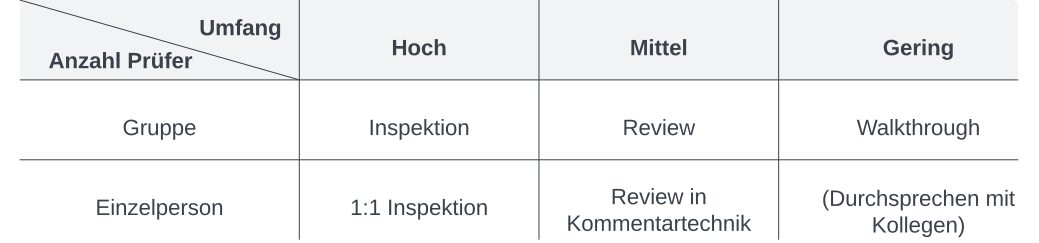
\includegraphics[scale=0.4]{part four/Manuelle Verfahren/img/manuelleverfahren}
    \caption{Verschiedene manuelle Verfahren, eingeordnet nach Anzahl der Teilnehmer und Umfang der Untersuchung. (Quelle: in Anlehnung an~\cite[Tab. 3.1, 17]{Wed09c})}
    \label{fig:manuelleverfahren-cc}
\end{figure}